%%%%%%%%%%%%%%%%%%%%%%%%%%%%%%%%%%%%%%%%%%%%%%%%%%%%%
%												    %
%	TROCA DE LETRAS		  						    %
%												    %
%	Maio 2015									    %
%												    %
%	Angela Cardodo e Bruno Madeira					%
%   											    %	
%%%%%%%%%%%%%%%%%%%%%%%%%%%%%%%%%%%%%%%%%%%%%%%%%%%%%

\documentclass[12pt,a4paper,reqno]{report}
\linespread{1.5}

\usepackage[active]{srcltx}    
\usepackage{graphicx}
\usepackage{amsthm,amsfonts,amsmath,amssymb,indentfirst,mathrsfs,amscd}
\usepackage[mathscr]{eucal}
\usepackage[active]{srcltx} %inverse search
\usepackage{tensor}
\usepackage[utf8x]{inputenc}
\usepackage[portuges]{babel}
\usepackage[T1]{fontenc}
\usepackage{enumitem}
\setlist{nolistsep}
\usepackage{comment} 
\usepackage{tikz}
\usepackage[numbers,square, comma, sort&compress]{natbib}
\usepackage[nottoc,numbib]{tocbibind}
%\numberwithin{figure}{section}
\numberwithin{equation}{section}
\usepackage{scalefnt}
\usepackage[top=2.5cm, bottom=2.5cm, left=2.5cm, right=2.5cm]{geometry}
%\usepackage{tweaklist}
%\renewcommand{\itemhook}{\setlength{\topsep}{0pt}%
%	\setlength{\itemsep}{0pt}}
%\renewcommand{\enumhook}{\setlength{\topsep}{0pt}%
%	\setlength{\itemsep}{0pt}}
%\usepackage[colorlinks]{hyperref}
\usepackage{MnSymbol}
%\usepackage[pdfpagelabels,pagebackref,hypertexnames=true,plainpages=false,naturalnames]{hyperref}
\usepackage[naturalnames]{hyperref}
\usepackage{enumitem}
\usepackage{titling}
\newcommand{\subtitle}[1]{%
	\posttitle{%
	\par\end{center}
	\begin{center}\large#1\end{center}
	\vskip0.5em}%
}
\newcommand{\HRule}{\rule{\linewidth}{0.5mm}}
\usepackage{caption}
\usepackage{etoolbox}% http://ctan.org/pkg/etoolbox
\usepackage{complexity}

\usepackage[official]{eurosym}

\def\Cpp{C\raisebox{0.5ex}{\tiny\textbf{++}}}

\makeatletter
\def\@makechapterhead#1{%
  %%%%\vspace*{50\p@}% %%% removed!
  {\parindent \z@ \raggedright \normalfont
    \ifnum \c@secnumdepth >\m@ne
        \huge\bfseries \@chapapp\space \thechapter
        \par\nobreak
        \vskip 20\p@
    \fi
    \interlinepenalty\@M
    \Huge \bfseries #1\par\nobreak
    \vskip 40\p@
  }}
\def\@makeschapterhead#1{%
  %%%%%\vspace*{50\p@}% %%% removed!
  {\parindent \z@ \raggedright
    \normalfont
    \interlinepenalty\@M
    \Huge \bfseries  #1\par\nobreak
    \vskip 40\p@
  }}
\makeatother


\begin{document}



\begin{titlepage}
\begin{center}
 
\vspace*{3cm}

{\Large Laboratório de Programação Orientada por Objetos}\\[2cm]

% Title
{\Huge \bfseries Batalha Naval \\[1cm]}

% Author
{\large Ângela Cardoso e Nuno Valente}\\[2cm]

\includegraphics[width=10cm]{feup_logo.jpg}\\[2cm]


% Bottom of the page
{\large \today}

\end{center}
\end{titlepage}

\tableofcontents


%%%%%%%%%%%%%%
% INTRODUCAO %
%%%%%%%%%%%%%%
\chapter{Introdução}

O trabalho desenvolvido foi realizado no âmbito da disciplina de Laboratório e Programação Orientada a Objetos – LPOO, unidade curricular do segundo ano do Mestrado Integrado em Engenharia Informática e Computação da Universidade do Porto.

O objetivo do trabalho foi escrever um programa com interface gráfica que permita ao utilizador jogar à batalha naval contra o computador ou contra outro jogador em rede. De futuro referir-nos-emos ao jogo da batalha naval simplesmente como jogo.

Pretende-se com a elaboração deste relatório descrever e justificar as opções escolhidas e apresentar os resultados obtidos com o término do programa/projeto.

Nos próximos pontos faremos a apresentação de um manual de utilização do jogo e abordaremos a forma como idealizamos a concepção e a implementação do jogo. Terminamos com a reflexão acerca do grau de cumprimento dos objetivos, as melhorias possíveis de se efetuar, além de referenciarmos a bibliografia consultada para apoio neste projeto.


%%%%%%%%
% JOGO %
%%%%%%%%
\chapter{O Jogo - Batalha Naval}

A batalha naval é um jogo de tabuleiro de dois jogadores, no qual os jogadores têm de desvendar em que quadrados estão os navios do adversário. Embora tenha sido o primeiro jogo em tabuleiro comercializado e publicado pela Milton Bradley Company em 1931, o jogo foi originalmente jogado com lápis e papel. O seu objetivo é afundar os navios do adversário. Ganha quem afundar todos os navios do adversário primeiro.

O jogo original é jogado em duas grelhas para cada jogador, uma que representa a disposição dos barcos do jogador, e outra que representa simultaneamente a do seu adversário e as suas tentativas. As grelhas são tipicamente quadradas, estando identificadas na horizontal por letras minúsculas e na vertical por letras maiúsculas. Em cada grelha o jogador coloca os seus navios e regista os tiros do oponente.

Antes do início do jogo, cada jogador coloca os seus navios nos quadrados, alinhados horizontalmente ou verticalmente. O número de navios permitidos é igual para ambos os jogadores e os navios não se podem sobrepor.

Após os navios terem sido posicionados o jogo continua alternadamente. Na sua vez um jogador aposta num quadrado na grelha do oponente, se houver um navio nesse quadrado, é colocada uma marca vermelha, senão houver é colocada uma marca azul, representando o tiro e a água, respetivamente.

Os tipos de navios são: porta-aviões (5 quadrados adjacentes), os submarinos (1 quadrado apenas), barcos de dois, três e quatro canos. Numa das variações deste jogo, as grelhas são de dimensão 10x10, e o número de navios são: 1, 4, 3, 2, 1, respetivamente.

%%%%%%%%%%
% MANUAL %
%%%%%%%%%%

\chapter{Manual de Utilização - CLI}

\section{Funcionalidades Suportadas}

	No interface de consola é possível iniciar um novo jogo ou continuar um jogo previamente gravado. Independentemente de se tratar de um novo jogo ou não, o jogador pode jogar sozinho (contra o computador) ou contra outro jogador.
	
	Caso se trate de um novo jogo, através da indicação de um ficheiro de configuração o jogador pode configurar o tamanho do tabuleiro e o tipo de navios. Uma vez configurado o jogo, cada jogador pode escolher a forma de posicionar os seus navios: manual ou automática. Em qualquer caso, após o posicionamento dos navios e antes do início do jogo, é permitido mudar a posição de qualquer navio.
	
	Durante o jogo, são alternadas as vezes de cada jogador. Em vez de jogar, o jogador pode escolher salvar o jogo e sair. Também é possível salvar o jogo num determinado ponto e continuar a jogar. Mais tarde, um jogo que seja retomado, dará a primeira vez ao jogador que interrompeu a sua vez e salvou o jogo.

	O jogo aguarda que cada jogador inicie a sua vez, garantindo assim que os tabuleiros permanecem ocultos do adversário.

\section{Modo de Utilização}
	
	Assim que inicia o jogo, o utilizador deve escolher entre iniciar um novo jogo ou carregar um jogo previamente gravado. Além disso, deve indicar também o número e o nome dos jogadores, assim como os ficheiros em que serão guardadas (ou lidas) as configurações de cada jogador.
	
	Se se tratar de um novo jogo, a fase seguinte é de colocação dos navios no tabuleiro. Cada jogador pode fazer isso de duas formas:
	\begin{itemize}
		\item manual - é escolhida a posição de cada navio, indicando a linha, a coluna e a orientação;
		\item automática - os navios são distribuídos aleatoriamente pelo tabuleiro.
	\end{itemize}
	Independentemente da forma de colocação, nesta fase é ainda possível alterar a posição de qualquer um dos navios.
	
	A fase seguinte é a fase de jogo. Se se tratar de um novo jogo, é sorteado o primeiro jogador. Caso contrário, juntamente com as restantes configurações, é também lido o jogador que tem o primeiro turno. Cada jogador tem a sua vez, escolhendo uma posição para atacar. Se o ataque for bem sucedido, isto é, se for atingido um navio do adversário, o jogador volta a atacar. A cada instante, o jogador vê o seu tabuleiro, assim como a sua visão do tabuleiro do adversário, de forma a poder jogar convenientemente.
	
	O jogo termina quando algum jogador afunda toda a frota do adversário, sendo mostrados ambos os tabuleiros e o vencedor.

\section{Formatos de ficheiros}

	Para que o jogo funcione na sua plenitude são necessários 3 ficheiros:
	\begin{itemize}
		\item um ficheiro de configuração, normalmente \emph{config.txt};
		\item um ficheiro para o jogador 1, normalmente \emph{board1.txt};
		\item um ficheiro para o jogador 2, normalmente \emph{board2.txt}.
	\end{itemize}
	
	O ficheiro de configuração indica na primeira linha o tamanho do tabuleiro no formato ``board - 10 x 10'', indicando que se trata de um tabuleiro com 10 linhas e 10 colunas. As linhas seguintes contêm a especificação de cada navio. Por exemplo, ``1 - Aircraft carrier - 5 - A - 255/0/255'', indica 1 navio de tipo \emph{Aircraft carrier}, com dimensão 5, símbolo \emph{A} e componentes RGB da cor $(255, 0, 255)$.
	
	Os ficheiros de cada jogador começam por indicar o tamanho de tabuleiro e o número de navios no formato ``10 - 10 - 7'', indicando 10 linhas, 10 colunas e 7 navios. Neste caso, as 7 linhas seguintes contêm cada um dos navios, por exemplo ``Aircraft carrier - A - 255/0/255 - 5 - Aa - H - false - true - true - true - true'' indica, relativamente ao primeiro navio, o tipo, o símbolo, a cor, a dimensão, a posição no tabuleiro, a orientação e de seguida o estado de cada célula: falso se estiver morta, verdadeiro se estiver viva. Após as linhas dos navios há uma linha com as dimensões do tabuleiro do adversário, que em princípio serão iguais. De seguida existe uma linha com as posições atacadas que revelaram água, por exemplo ``Aj'' indica que foi atacada a primeira linha e última coluna sendo obtida água. A linha das posições que revelaram ataques bem sucedidos é a seguinte, por exemplo ``Aa - Ba'' indica que foram atacadas com sucesso duas posições. Finalmente a última linha indica se é a vez desse jogador \emph{true} ou não \emph{false}. 

\chapter{Manual de Utilização - GUI}

\section{Funcionalidades Suportadas}

\section{Modo de Utilização}

\subsection{Ecrã Inicial}

\begin{center}

\includegraphics[width=16cm]{ecrainicial.jpg}

\end{center}

Ao iniciar o jogo é apresentado no ecrã a janela de entrada no jogo, com áudio ativo. Nessa janela é possível começar um novo jogo, em \emph{Start Game}, carregar um jogo previamente gravado, em \emph{Load Game}, consultar a ajuda disponível em \emph{Help}, ou então simplesmente desligar o jogo carregando em \emph{Quit}.

Antes de iniciar o jogo o utilizador poderá aceder ao menu \emph{Help}, consultando aí a forma de jogar, informação sobre o projeto e seus autores.

É possível navegar nestes menus através das teclas direcionais do teclado, premindo \emph{Enter} caso seja a opção pretendida, ou então com um simples clique do rato.

\subsection{Ecrã de Configuração}

\begin{center}

\includegraphics[width=16cm]{configuracao.jpg}

\end{center}

No ecrã de configuração temos a hipótese de selecionar um jogo contra o computador ou contra outra pessoa. Fornecemos também a possibilidade de carregar as configurações de um jogo começando um novo jogo com colocação automática dos navios no tabuleiro. Neste ecrã permitimos que o jogador ou os jogadores coloquem o seu nome para posteriormente aparecer no tabuleiro de jogo.

\subsection{Ecrã de Jogo}

\begin{center}

\includegraphics[width=16cm]{ecradejogo.jpg}

\end{center}

No ecrã de jogo, onde toda a mecânica de jogo se desenrola, decidimo-nos por 2 painéis de jogo. No painel da esquerda, temos os navios já colocados por parte de um jogador. No painel da direita, temos as tentativas de acerto nos navios do adversário.

Na barra inferior desta janela, era nossa intenção colocar as estatísticas em tempo real de cada jogador, embora não tenhamos terminado essa tarefa.

\section{Formatos de ficheiros}

	Os ficheiros de texto são iguais independentemente do interface.

%%%%%%%%%%%%%%%%
% INTELIGENCIA %
%%%%%%%%%%%%%%%%
\chapter{Inteligência Artificial}

	Quando jogado por um único jogador, o jogo possui uma inteligência artificial para jogar a vez do adversário. Este jogador começa por atacar posições aleatórias no tabuleiro do adversário, garantindo que não ataca duas vezes a mesma célula. Em caso de sucesso de um ataque, as próximas posições serão as células vizinhas, para tentar afundar todo o navio.
	
	Apesar de a técnica de atacar a vizinhança não ser exatamente aquilo que faz um bom jogador humano, que tenta também perceber qual o formato do navio que está a atacar, o desempenho desta inteligência artificial é razoável. Em situações em que os navios estejam próximos uns dos outros, este jogador tem um desempenho especialmente bom.

\chapter{Concepção e Implementação}


\section{Estrutura de Packages}

\begin{center}

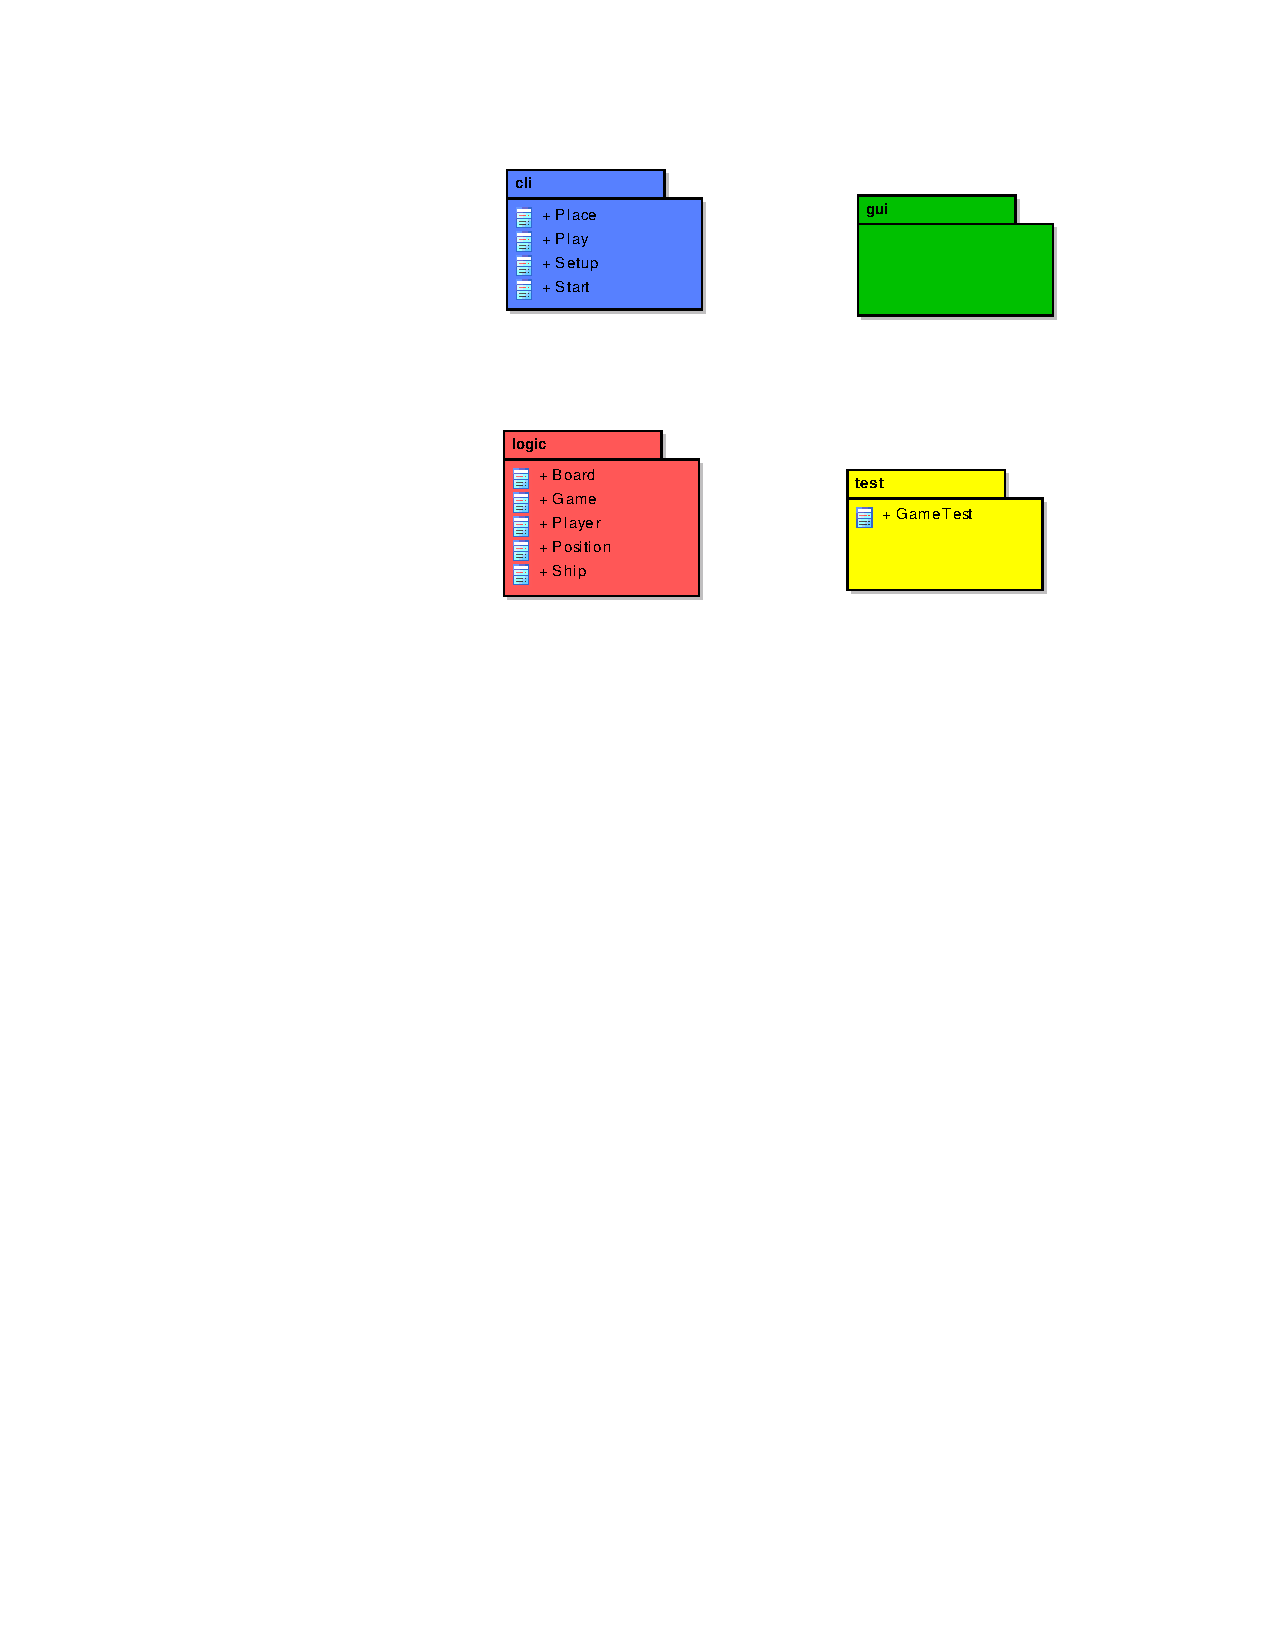
\includegraphics[width=16cm]{package.jpg}

\end{center}

\section{Estrutura de Classes}

\begin{center}

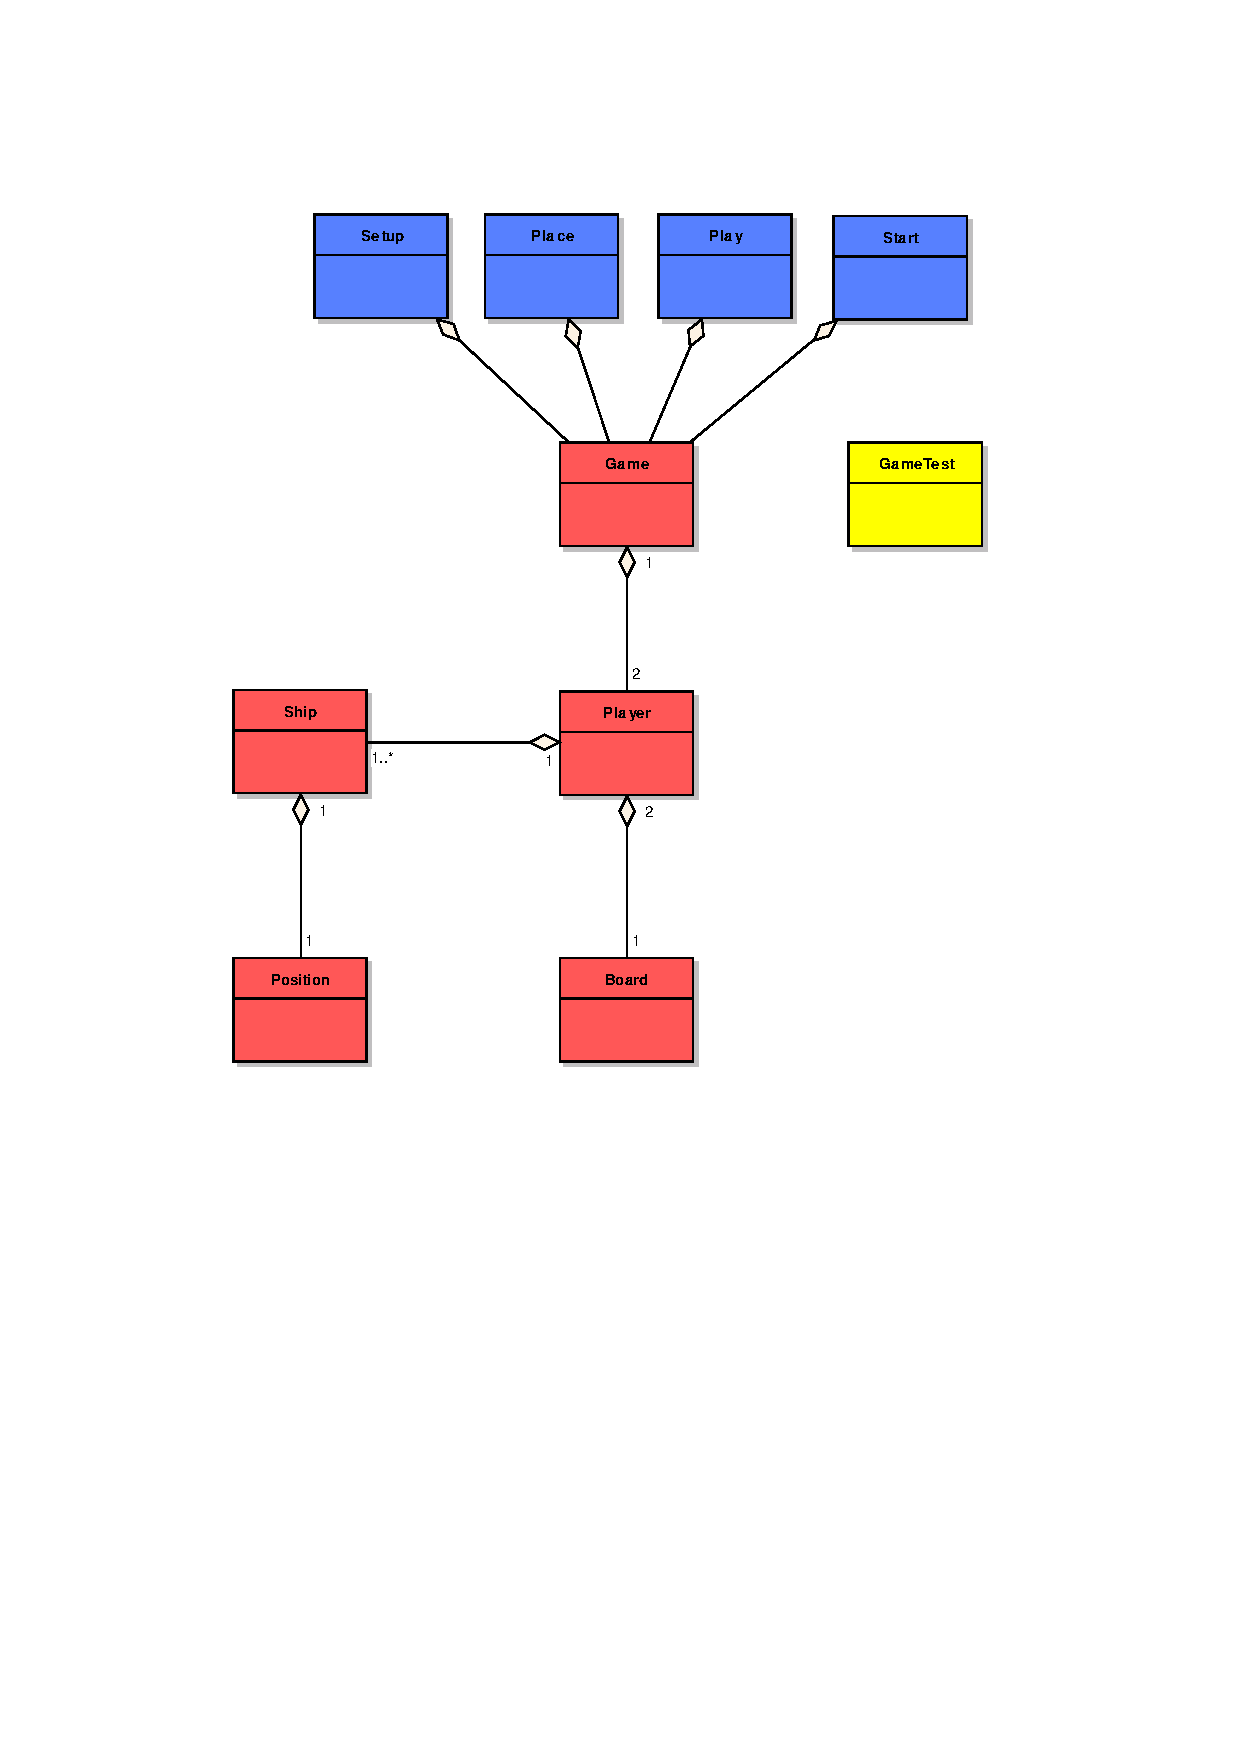
\includegraphics[width=16cm]{class.jpg}

\end{center}

\section{Padrões de Desenho Utilizados}

	Utilizamos o padrão \emph{singleton} para garantir que existe uma única instância de jogo e também para garantir que existe uma única instância de cada posição de tabuleiro consoante as suas coordenadas.

%%%%%%%%%%%%%
% CONCLUSAO %
%%%%%%%%%%%%%
\chapter{Conclusões}

\section{Grau de Cumprimento dos Objectivos}
	
	Por falta de tempo, não implementamos o servidor que permitiria jogar em rede. Além disso, o interface gráfico também está relativamente incompleto. Os restantes aspetos do jogo estão terminados.

\section{Melhorias Possíveis}

	Em vez de utilizar um ficheiro de configuração, seria interessante permitir configuração do jogo nos interfaces. Além disso, a inteligência artificial poderia ser melhor, ou então o jogo poderia ter níveis de dificuldade e mais do que uma inteligência artificial.

\section{Distribuição do Trabalho}
	
	Os elementos do grupo, sendo este constituído por dois alunos, contribuíram com o seu trabalho, empenho e dedicação no desenvolvimento do projeto na mesma proporção.

\end{document}
